\section{Technika sítí a protokolů - komunikační modely, způsob přenosu informace, základní struktura sítí, typy sítí, architektura komunikace systémů.}
\label{q01}

\subsection{Komunikační modely}

Komunikaci mezi dvěma stranami lze rozlišit na~dva typy: \textbf{komunikaci uvnitř sítí} a~\textbf{komunikaci mezi koncovými uživateli} (nad~sítěmi).

\textbf{Data} jsou reprezentace faktů, pojmů nebo instrukcí ve~formální podobě vhodná pro~komunikaci a~interpretaci pro~strojové zpracování. \textbf{Informace} je význam dat, důležitý typicky pro~uživatele.

\begin{figure}[ht]
	\centering
	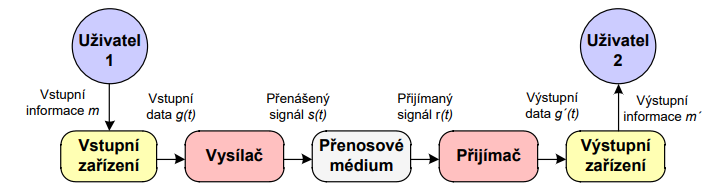
\includegraphics[width=\textwidth]{images/q01_simplified_scheme_network}
	\caption
		[Zjednodušené blokové schéma datovké komunikace]
		{Zjednodušené blokové schéma datovké komunikace. \\
		Informace $m$ je pomocí vstupního zařízení reprentována jako data $g(t)$ ve~formě proměnlivého časového signálu, který musí být přeložen do~podoby vhodné pro~přenosové médium, tj. do~signálu $s(t)$, vysílačem. Na~druhé straně se objeví jako signál $r(t)$, který se od~odeslaného může odlišovat (šum, rušení). Je konvertován zpět do~tvaru výstupních dat $g'(t)$ a~výstupnímu zařízení jsou předána data $m'$.}
	\label{q01_simplified_scheme_network}
\end{figure}

Pomocí komunikačních sítí spolu komunikují koncoví uživatelé, v~případě počítačů partnerské procesy na~komunikujících počítačích. Základním předpokladem pro~komunikaci uživatelů je definice rozhraní mezi~uživatelem a~sítí; musí konkretizovat strukturu a~formát předávaných uživatelských a~řídících dat.

\begin{figure}[ht]
	\centering
	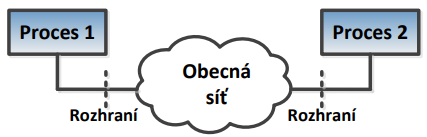
\includegraphics[width=0.5\textwidth]{images/q01_simplified_scheme_processes}
	\caption{Zjednodušené blokové schéma komunikace mezi procesy pracujícími na~samostatných počítačích propojených obecnou sítí.}
	\label{q01_simplified_scheme_processes}
\end{figure}

Základní úkoly pro~přenos informace spočívají ve~vlastním \textbf{přenosu} informace (kódování dat a~jejich přizpůsobení pro~telekomunikační kanál), vyhledání cesty spojení dvou uživatelů v~síti (\textbf{směrování}) a~použití vhodného způsobu komunikace a~řízení (\textbf{protokoly}).

Komunikační řetězec zejména stará o~\textbf{řízení výměny} informací (způsob organizace přenosu dat mezi zdrojem a~cílem), \textbf{definice rozhraní} (včetně tvaru a~velikosti signálu), \textbf{synchronizaci} (časové sjednocení), \textbf{formátování zpráv} (unifikace způsobu sestavení obsahu zprávy) a~\textbf{adresování a~směrování} (jednoznačný způsob určení cíle a~nalezení cesty k~němu).

Zpravidla umožňuje vícenásobné využití přenosových systémů (sdílení více uživateli/procesy), \textbf{řízení systému} (konfigurace, dohled, reakce na~chyby a~přetížení), \textbf{detekci a~korelaci chyb}, \textbf{zotavení} se ze~ztrát v~komunikačním systému, \textbf{řízení přenosu} (aby nedocházelo k~zahlcení systému nadměrným množstvím dat) a~ochranu zpráv (zaslaná data může přijímat pouze příjemce).

\subsection{Přenos informace}

Při~přenosu hovoru jsou mezi částmi přenášenené informace malé mezery, jde o přenos citlivý na~zpoždění a~má vysokou nadbytečnost. Přenos dat na~počítači je naopak převážně dávkový, velmi spolehlivý a~existence spojení není až tak kritická.

\paragraph{Komutace okruhů (Circuit Switching)} Mezi koncovými účastníky je vytvořena dočasná přenosová cesta jako fyzické spojení (včetně spojovacích uzlů). Spojení je nutné sestavovat před~vlastním přenosem informace, je potřeba rezervovat prostředky a~kapacity pro~následný přenos. Z~hlediska nákladů jde o~drahé spojení: cesta je vytížená i~když k~přenosu informace dochází pouze část alokované doby. Využívaná dříve pro~přenos telefonních hovorů.

\paragraph{Komutace zpráv (Message Switching)} Zdroj informace vyšle zprávu do~prvního uzlu, kde se uloží, zkontroluje a~pošle k~dalšímu uzlu směrem k~příjemci dat. Tento způsob klade velké nároky na~mezilehlé uzly (musí být schopny zprávy uchovat v~paměti; \emph{store-and-forward}). Vždy je zatěžována pouze ta část sítě po~které se zpráva přenáší.

\paragraph{Komutace paketů (Packet Switching)} Zpráva je rozdělena na~bloky dat (pakety) o~definované maximální délce, sítí jsou přenášeny stejně jako zprávy. Pořadí doručení paketů nemusí být dodrženo, tato metoda vyžaduje dodatečné prostředky pro~zajištění správnosti přenesení celé zprávy (pouhé protichybové zabezpečení již nestačí). Jde o~nejčastější způsob přenosu.

\paragraph{Komutace buněk (Cell Switching)} Zpráva je rozdělena na~jednotky s~přesně danou délkou. Při~přenosu se provádí pouze kontrole záhlaví buňky/rámce a~proto dochází jen k~velmi malému zdržení v~uzlu. Veškeré kontroly přenesených dat jsou prováděny u~koncového uživatele. Využívá se u~přenosu řeči i~u~klasických dat (ATM technologie%
\footnote{Asynchronous Transfer Mode: \url{https://en.wikipedia.org/wiki/Asynchronous_Transfer_Mode}.}%
). Dochází k~velké úspoře prostředků sítě, protože je blokována pouze nezbytná kapacita, a~k~urychlení odezvy, nevýhodou je však zmíněná fixní velikost přenášených jednotek.

\begin{figure}[ht]
	\centering
	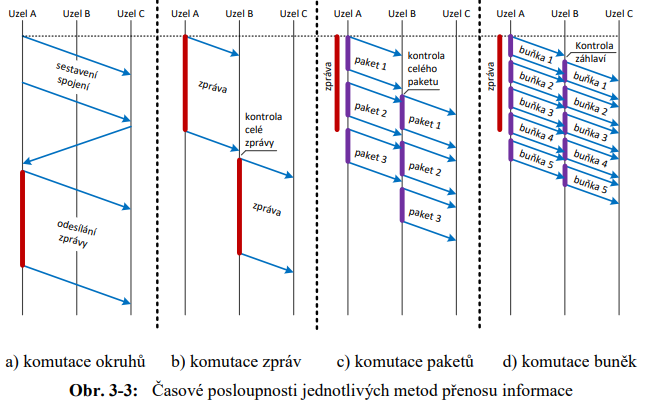
\includegraphics[width=0.9\textwidth]{images/q01_switching}
	%\caption{Časové posloupnosti jednotlivých metod přenosu informace}
\end{figure}

\subsection{Struktura sítí}

\textbf{Spoje} jsou komponenty umožňující přenos zpráv mezi dvěma místy bez~ohledu na~druh prostředků či~druh přenosu a~propojují přepojovací prvky mezi sebou a~s~koncovými uzly. Jde o~okruhy, kanály nebo linky.

\textbf{Přepojovací prvky} jsou specializované systémy sloužící k~propojení dvou a~více spojů. Základní úlohou je vybrání správného výstupního spoje po~kterém budou data poslána dále. Pro~datové přenosy je to IMP (\emph{Interface Message Processor}), předchůdce směrovačů v~TCP/IP%
\footnote{Pro~IMP se také používají názvy datová ústředna (\emph{Data Switching Exchange}), mezilehý systém (\emph{Intermediate System}) nebo uzel přepojování paketů (\emph{Packet Switching Node}).}.

\begin{figure}[ht]
	\centering
	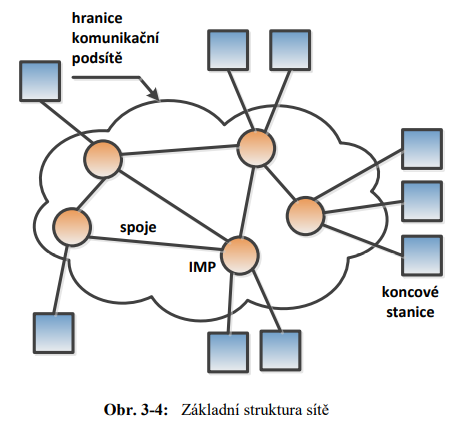
\includegraphics[width=0.4\textwidth]{images/q01_imp}
	%\caption{Základní struktura sítě}
\end{figure}

\subsubsection{Architektura a~topologie sítí}

\textbf{Dvoubodové spoje} informace vyměňují nepřímo. Mezi možné struktury patří topolotie typu stromhvězda, kruh, strom, polygon, propojené kruhy nebo~může jít o~obecnou topologii (neúplný polygon).

\begin{figure}[ht]
	\centering
	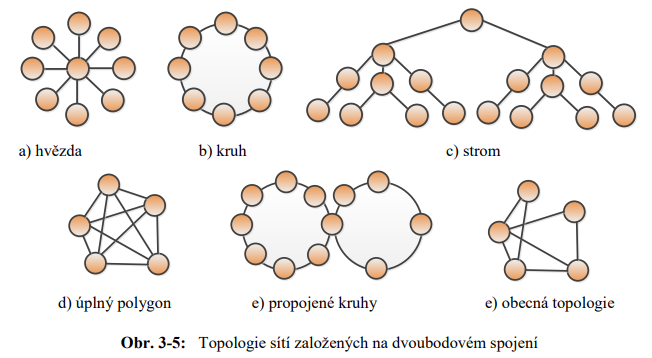
\includegraphics[width=0.6\textwidth]{images/q01_network_topology}
	%\caption{Topologie sítí založených na~dvoubodovém spojení}
\end{figure}

\textbf{Multipoint} je topologické uspořádání ve~kterém může být vytvořeno více kanálů mezi dvěma místy. \textbf{Broadcast} je hromadný přenos z~jednoho zdroje do~mnoha míst. Spadají sem převážně bezdrátové sítě: systémy mají jeden kanál který je využívaný všemi uživateli. Vyslaná data jsou přijmuta všemi, reaguje na~ně obvykle pouze ten komu byla zaslána. Systémy se~všesměrovým vysíláním také umožňují adresovat skupinu nebo všechny stroje pomocí speciálních adres (multicast).

\begin{figure}[ht]
	\centering
	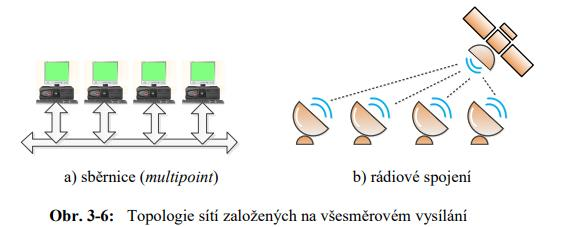
\includegraphics[width=0.5\textwidth]{images/q01_multipoint_topology}
	%\caption{Topologie sítí založených na~všesměrovém vysílání}
\end{figure}

\subsection{Typy sítí}

Nejčastěji se sítě dělí dle velikosti, dosahu nebo rozlohy. Některá řešení je obtížné zařadit do~jedné konkrétní kategorie.

\paragraph{Personal Area Network (PAN)} Využívá se pouze jednou osobu (příp. velmi nízkým počtem osob), zpravidla nízkými přenosovými rychlostmi (Mbps), často bezdrátově (Bluetooth, IrDA%
\footnote{IrDA: Infrared Data Association}%
, ale i~USB). Chytré telefony, PDA, tablety, scannery, tiskárny.

\paragraph{Local Area Network (LAN)} Přenos informací v~prostorově omezeném měřítku (budova až~jednotky kilometrů). Obvykle v~provedení hvězda nebo strom. Rychlosti 100 Mbps až~10 Gbps. Uzlů bývají desítky až~stovky. Doba zpoždění přenosu se pohybuje od~10~\si{\micro s} do~1~ms. Domácnosti, firmy, budovy ve~vlastnictví jedné osoby nebo organizace.

\paragraph{Metropolitan Area Network (MAN)} Propojení LAN sítí s~WAN sítěmi. Rozsah měst až~národních sítí. Rychlosti v~řádu Gbps a~vyšších. Optické technologie, Ethernet v~optických vláknech, dříve také ATM či FDDI%
\footnote{FDDI: Fiber Distributed Data Interface.}%
. MAN sítě jsou spravovány jednou organizací a~její prostředky jsou využívány více subjekty. Zpoždění přenosu se~pohybuje od~100 \si{\micro s} do~10~ms.

\paragraph{Wide Area Network (WAN)} Globální sítě pokrývající stovky až tisíce kilometrů na~úrovni států či~kontinentů. Jejich hlavní úlohou je~propojení geogreficky rozprostřených LAN a~MAN sítí. Jedna WAN může být vystavena na~více technologiích a~její části mohou být vlastněny různými subjekty. Přepínání pektů, buněk i~okruhů; technologie POS%
\footnote{POS: Packet over SONET/SDH (Synchronous Optical Network/Synchronous Digital Hierarchy).}%
, MPLS%
\footnote{MPLS: Multiprotocol Label Switching}%
, ATM či~Frame Relay. Využívají se převážně optické technologie. Zpoždění bývá vhledem k~velkým vzdálenostem vyšší (navzdory přenosu rychlostí světla), řádově jednotky až~stovky ms. Nejpoužívanější WAN sítí je Internet.

\subsection{Architektura komunikace systémů}

Přenos mezi stranami vždy probíhá dle dohodnutých pravidel (\textbf{protokolu}).

\textbf{Vertikální komunikace} probíhá od~nejvyšší úrovně k~nejnižší a~naopak. Pro~obě strany je transparentní, probíhá ale přes všechny úrovně systému.

\textbf{Horizontální komunikace} probíhá na~odpovídajících úrovních domluveným protokolem, a~s~výjimkou fyzické vrstvy je pouze virtuální. Každá vrstva musí umět předat data nižší vrstvě a~také od~ní data převzít a~\enquote{očistit} je pro~předání výše.

\begin{figure}[ht]
	\centering
	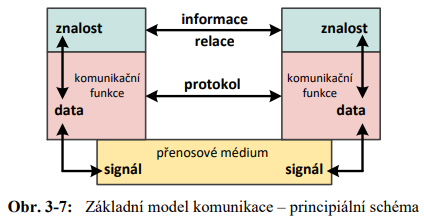
\includegraphics[width=0.7\textwidth]{images/q01_communication_architecture}
\end{figure}

\clearpage
\section{Základní popis referenčního modelu ISO/OSI a srovnání s TCP/IP.}

Na~počátku mezipočítačové komunikace vznikaly různé vzájemně nekompatibilní systémy a~uzavřené architektury. Postupem času rostl tlak na~vznik otevřeného standardu, který byl standartizován jako ISO/OSI RM%
\footnote{International Organization for Standartization Open System Interconnection Reference Model.}%
, který podchycuje všechny nezbytné aspekty komunikace. Stal se výchozím modelem pro~počítačově řízenou výměnu dat a~položil teoretický a~vědecký základ pro~realizaci datových sítí.

Zařízení vykonávající zpracování a~přenos informace jsou označovány jako \textbf{reálné systémy}, prvky zpracovávající informace jsou \textbf{aplikační procesy}.

ISO/OSI RM nespecifikuje přesnou podobu sítě, ale uvádí všeobecné principy sedmivrstvé síťové architektury. Jsou to:

\begin{enumerate}
	\item fyzická (\emph{physical}) vrstva,
	\item spojová (\emph{data link}) vrstva ,
	\item síťová (\emph{network}) vrstva,
	\item transportní (\emph{transport}) vrstva,
	\item relační (\emph{session}) vrstva,
	\item prezentační (\emph{presentation}) vrstva,
	\item aplikační (\emph{application}) vrstva.
\end{enumerate}

Nejnižší dvě vrstvy bývají \textbf{hardwarové}, ostatní bývají implementovány \textbf{softwarově}.

První čtyři vrstvy lze označit jako \textbf{poskytovatele} transportní služby, třetí až~sedmou jako jejího \textbf{uživatele}.

První tři vrstvy jsou \textbf{lokální}, protože zajišťují komunikaci na~lokální síťové infrastruktuře, čtyři vrchní jsou \textbf{koncové} a~umožňují propojení komunikujících aplikací.

Datové jednotky se označují jako PDU (\emph{Protocol Data Unit}) a~každá vrstva má své označení: TPDU (\emph{Transport PDU}), SPDU (\emph{Session PDU}), PPDU (\emph{Presentation PDU}), APDU (\emph{Application PDU})).

Partnerská komunikace vrstev je pouze iluze, data prochází všemi nižšími vrstvami. V~mezilehém prvku dochází k~průchodu do~síťové vrstvy, kde je rozhodnuto o~dalším směrování a~následně data \enquote{sestoupí} k~fyzické vrstvě.

\begin{figure}[ht]
	\centering
	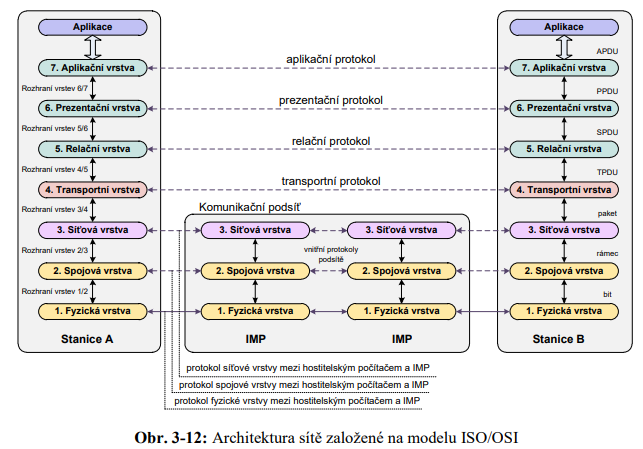
\includegraphics[width=\textwidth]{images/q02_iso_osi}
	%\caption{Architektura sítě založené na~modelu ISO/OSI}
\end{figure}

Sestupem do~nižší vrstvy se zvyšuje datová jednotka o~záhlaví jednotlivých vrstev (tzv. \textbf{zapouzdřování}). V~cílovém systému se v~jednotlivých vrstvách zprávy rozbalují.

\begin{figure}[ht]
	\centering
	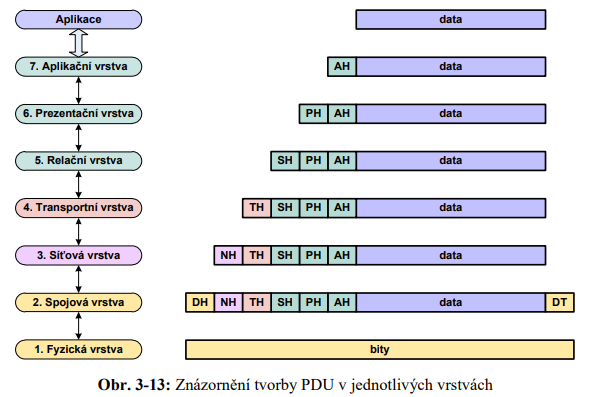
\includegraphics[width=0.7\textwidth]{images/q02_iso_osi_pdu}
	%\caption{Tvorba PDU v~jednotlivých vrstvách}
\end{figure}

\subsection{Vrstvy modelu ISO/OSI}

Aplikační procesy rozptýlené po~síti mezi sebou komunikují. Logické prostředí sítě je pro~uživatele transparentní.

\paragraph{Fyzická vrstva} Jde o~prostý tok bitů přenosovým médiem (tj. přenos elektrického signálu s~měnícími se napěťovými úrovněmi). Úkolem první vrstvy je příprava funkčních, procedurálních, mechanických a~elektrických prostředků pro~vytvoření, udržení a~ukončení datových okruhů mezi prvky sítě. Kvalita je popisována \textbf{chybovostí}.

Reprezentace bitů, přenosová rychlost, synchronizace vysílače s~přijímačem, přizpůsobení se kanálu a~topologii, oboustranný přenos.

\paragraph{Spojová vrstva} Přenášení rámců. Druhá vrstva připravuje prostředky pro~vytvoření, udržení a~rušení datových spojů mezi dvěma prvky sítě, mezi kterými může být jedno či~více spojení, které vznikají a~zanikají dynamicky. Krom práce s~datovými spoji tato vrstva formátuje rámce, identifikuje koncové body, řadí přenášené rámce, detekuje a~opravuje chyby a~oznamuje chyby které nezvládá opravit.

Podvrstva řízení logického spoje (LLC, \emph{Logical Link Control}) poskytuje rozhraní mezi přenosovým prvkem a~síťovou vrstvou, podvrstva řízení přístupu k~médiu (MAC, \emph{Media Access Control}) poskytuje služby specifické pro~daný přenosový prostředek.

Vytváření rámců, adresování v~síti, řízení toku dat, řízení chybových stavů.

\paragraph{Síťová vrstva} Směrování toku dat organizovaných do~paketů. Třetí vrstva poskytuje prostředky pro~transportní jednotky. Je zodpovědná za~komunikaci na~základě logických adres, směrování a~přenos datových jednotek (datagram) k~přijímači. Zajišťuje hlavně nezávislost transportní vrstvy na~směrování a~propojování, dále také síťovou adresaci, management síťových spojů, prioritizaci přenosu nebo řazení datagramů.

Může být \textbf{se~spojením} nebo \textbf{bez~spojení}. Směrování je vyhledání optimální cesty k~cíli. Síťová vrstva také musí mít mechanismus mapování logických adres na~fyzické.

Logické adresování, směrování mezi sítěmi.

\paragraph{Transportní vrstva} Zvýšení kvality spojů na~požadovanou úroveň: vyšší vrstvy nemusí určovat optimální cestu, kontrolovat tok dat nebo řešit problémy s~přetížením či~chybami. Prototoly čtvrté a~vyšší vrstvy pracují v~koncových systémech. Koncové body transportního přenosu jsou odlišeny pomocí \textbf{portů}. \textbf{Kvalita služeb} závisí na~přenášených datech.

Adresace konkrétní služby, segmentace a~skládání, řízení spojení, toku dat a~chybových stavů.

\paragraph{Relační vrstva} Informace pro~řízení a~synchronizaci dialogu. Pátá vrstva organizuje a~synchronizuje dialog aplikačních procesů. V~rámci jedné relace může vzniknout více transportních spojení, více transportních spojení může reprezentovat jednu relaci.

Řízení dialogu aplikačních protokolů, synchronizace.

\paragraph{Prezentační vrstva} Koordinace kódování a~syntaxe vyměňovaných dat. Šestá vrstva transformuje data aplikační vrstvy do~společného formátu: převod kódů a~abeced či uspořádání dat. V~ISO/OSI modelu je jedinou vrstvou která může zasahovat do~samotných přenášených dat. Data může také komprimovat či~šifrovat.

Transformace kódování, šifrování, komprese.

\paragraph{Aplikační vrstva} Informačním systémům zpřístupňuje prostředí OSI. Sedmá vrstva se dá nazvat jako síťové rozšíření operačního systému. Zajišťuje přenos zpráv, identifikaci partnerů, zjišťování připravenosti partnera, určení kvality služeb, zajištění synchronizace zpráv, dohodu syntaxe apod.

Příklady jsou například přenos souborů, elektronická pošta nebo vzdálený přístup, které jsou dnes využívány pouze nad TCP/IP.

\clearpage
\section{Základní popis síťového modelu TCP/IP a~srovnání s~ISO/OSI.}

Navzdory názvu TCP/IP označuje celou sadu protokolů a~náhledů na~stavění a~fungování datových sítí. Na~rozdíl od ISO/OSI je praktická pro~reálnou implementaci.

Při~vytváření RM OSI měly hlavní slovo organizace kladoucí důraz na~vlastnosti sítě (na~jejich spojovaný a~spolehlivý charakter) s~tím, že připojované hostitelské počítače nebudou muset provádět tolik práce. Vyšší vrstvy ale nemohly spoléhat na~opravy vrstev vyšších a~spolehlivost si musely zajišťovat samy, a~ve výsledku se tím zabývala každá vrstva.

Tvůrci TCP/IP naopak vycházeli z~předpokladu, že zajištění spolehlivosti je problémem koncových zákazníků a~mělo by být řešeno až na~úrovni transportní vrstvy a~výše. Komunikační síť nemusí ztrácet část přenosové kapacity kontrolou a~opakovaným vysíláním paketů a~je tak plně využita vlastními datovými přenosy. V~síti může dojít ke~ztrátě či zahození paketu bez varování a~snahy o~nápravu, pakety by však neměly být zahazovány bezdůvodně (naopak by se o~doručení měly snažit: \emph{best effort}). \textbf{TCP/IP předpokládá jednoduchou a~rychlou podsíť ke~které se připojují inteligentní počítače}.

\begin{figure}[ht]
	\centering
	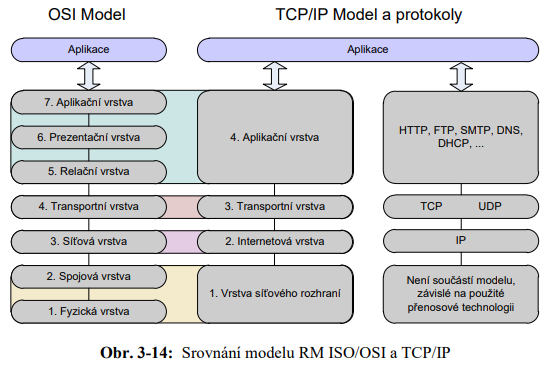
\includegraphics[width=\textwidth]{images/q03_osi_tcp}
	%\caption{Srovnání modelu ISO/OSI a~TCP/IP}
\end{figure}

\subsection{Vrstvy modelu TCP/IP}

\paragraph{Vrstva síťového rozhraní} Ovládání konkrétní přenosové cesty mezi dvěma síťovými prvky. Není blíže specifikována protože je závislá na~přenosové technologii.

\paragraph{Internetová vrstva} Realizace protokolem IP (v4, v6). Funkčně odpovídá síťové vrstvě ISO/OSI modelu a~bývá tak i~označována. Předává pakety mezi odesílatelem a~příjemcem přes mezilehá zařízení (směrovače). Jde o~nespojovanou datagramovou službu, která se musí vyrovnávat s~odlištnostmi částí cesty (odlišné adresy, různá maximální velikost paketů).

\paragraph{Transportní vrstva} Zajištění přenosu mezi dvěma koncovými účastníky (aplikačními programy). Podle nároků reguluje tok dat oběma směry, zajišťuje spolehlivost přenosu a~mění nespojovaný charakter internetové vrstvy na~spojovaný. Bývá realizována spolehlivým protokolem TCP (\emph{Transmission Control Protocol}), nespolehlivým UDP (\emph{User Datagram Protocol}) nebo i~jinými.

\paragraph{Aplikační vrstva} Případné prezentační a~relační služby (šifrování, komprese) si musí aplikace realizovat samy (a~pokud je aplikace nevyžaduje, nevzniká zbytečná režie). Mezi hlavní protokoly patří DNS, DHCP, HTTP, SSH, FTP, \dots

\subsection{Propojování sítí}

TCP/IP usiluje o~co nejuniverzálnější propojení sítí všech typů: od~lokálních typu Ethernet přes~veřejné datové sítě až po~internet. Cílem je umožnit každému uzlu komunikovat s~kterýmkoliv jiným uzlem bez ohledu na~to, jestli mezi nimi existuje přímé spojení, nebo jsou odděleny několika sítěmi.

Z~pohledu uživatele by vnitřní struktura soustavy měla být transparentní a~\emph{internetworking} by se jim měl jevit jako jedna velká síť, ke~které jsou připojeny jednotlivé počítače (\emph{hosts}). Ve~skutečnosti je to ale spousta dílčích sítí vzájemně propojených na~úrovni síťové vrstvy pomocí směrovačů (\emph{router}).

Výhodou IP je existence jednotého formátu adres, adresování a~dat na~úrovni síťové vrstvy.

\begin{figure}[ht]
	\centering
	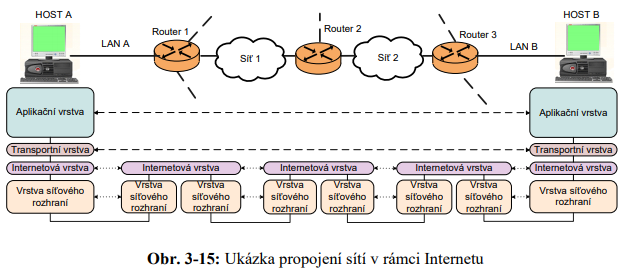
\includegraphics[width=\textwidth]{images/q03_internet}
	%\caption{Ukázka propojení sítí v~rámci internetu}
\end{figure}

Každé zařízení má fyzickou adresu spjatou s~konkrétním hardware. Pomocí MAC nelze komunikovat mezi různými sítěmi, proto jsou definovány globálně platné IP adresy.

\clearpage
\section{Principy komunikačních technik -- vícenásobné využití cest, zajištění obousměrné komunikace.}

Nejlepšího ekonomického zhodnocení přenosových cest se dosáhne jejich vícenásobným využitím. Pro~to se využívají techniky multiplexování, kdy je přes jedno médium přenášeno více signálů z~více zdrojů do~více cílů. Techniky multiplexování se často kombinují.

\paragraph{Prostorové dělení} \emph{Space-Division Mutliplex} je např. více paralelních vedení v~rámci jednoho kabelu; toto však není pravé multiplexování.

\paragraph{Kmitočtové dělení} \emph{Frequency-Division Multiplex} pro~různé přenosy využívá různé kmitočty, resp. pásma kmitočtů. Typickým příkladem je FM rádio nebo GSM. Z~FDM vychází OFDM (\emph{Orthogonal FDM}), které využívá například xDSL%
\footnote{xDSL: Digital Subscriber Line.}%
. Kmitočtové dělení může být také použito k~odlišení směrů komunikace (jedno pásmo tam, druhé zpět).

\begin{figure}[ht]
	\centering
	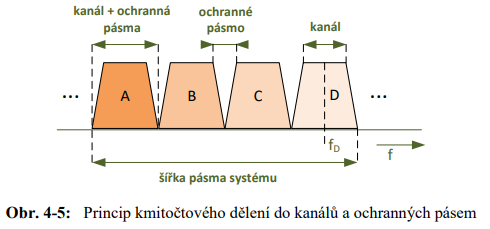
\includegraphics[width=0.7\textwidth]{images/q04_frequency}
	%\caption{Kmitočtové dělení do~kanálů a~ochranných pásem}
\end{figure}

\paragraph{Vlnové dělení} \emph{Wavelength-Division Multiplex} se využívá v~optice: v~jednom optickém vlákně je více signálů odlišených vlnovou délkou (barvou).

\paragraph{Časové dělení} \emph{Time-Division Multiplex} se využívá především v~digitálním přenosu, kdy se vysílací strany střídají.

V~\textbf{synchronním} módu je každému zařízení vyhrazeno $\frac{1}{n}$ celkové kapacity: když stanice nevysílá, blokuje svou alokovanou část a~přenos se stává neefektivním, všechny stanice také musí odesílaná data fragmentovat na~přesně dané a~stejně velké jednotky.
v~\textbf{asynchronním} módu jsou stanoveny časové intervaly s~přesně danou velikostí, ale nejsou nikým rezervované a~použity jsou pouze v~případě potřeby.
V~\textbf{paketovém} módu je možné vysílat různě velké zprávy v~libovolném čase. Každá zpráva musí obsahovat záhlaví s~identifikátorem vysílací stanice. Systém však nezaručuje žádnou vysílací kapacitu.

\begin{figure}[ht]
	\centering
	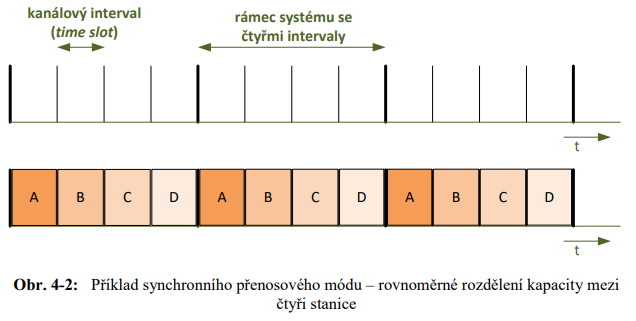
\includegraphics[width=0.7\textwidth]{images/q04_time_synchronous}
	%\caption{Synchronní přenosový mód}
	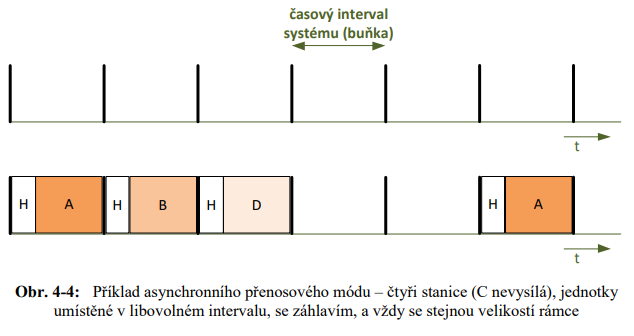
\includegraphics[width=0.7\textwidth]{images/q04_time_asynchronous}
	%\caption{Asynchronní přenosový mód}
	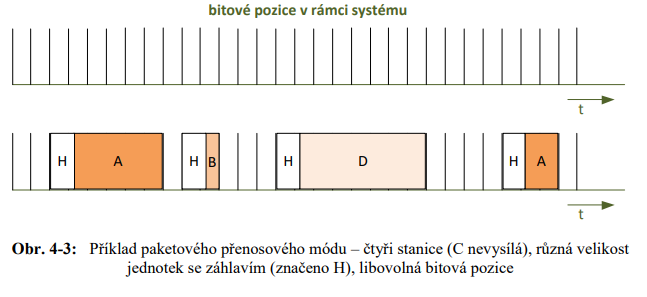
\includegraphics[width=0.7\textwidth]{images/q04_time_packet}
	%\caption{Paketový přenosový mód}
\end{figure}

\paragraph{Kódové dělení} \emph{Code-Division Multiplex} jednotlivé přenosy odlišuje speciální kódovou sekvencí.

\subsection{Metody zajištění obousměrné komunikace}
\label{q07}

\textbf{Simplexní spojení} umožňuje obousměrnou komunikaci, ale ne v~jednom okamžiku zároveň; protistrany se o~přenosovou kapacitu musí dělit. Jsou to například vysílačky, kde si komunikující musí slovně předávat signál že dohovořili.

\textbf{Duplexní spojení} umožňuje současnou komunikaci oběma směry. V~nejjednodušším případě existuje mezi oběma stanicemi dvojice kanálů, u~rádiových přenosů se \emph{full-duplex} emuluje časovým nebo frekvenčním dělením.

\clearpage
\section{Fyzická vrstva přenosových systémů -- přenosová média, analogové a digitální modulace, klíčovací techniky, princip digitalizace řečového signálu.}

\clearpage
\section{Spojová vrstva přenosových systémů -- podvrstvy, rámce spojové vrstvy, adresace, metody zajištění spolehlivého přenosu.}

\clearpage
\section{Síťová vrstva přenosových systémů -- spínání paketů, služby síťové vrstvy, IPv4 adresy, techniky směrování, IPv4 datagram.}

\subsection{Přepojování paketů}

Síťová vrstva hledá optimální cestu mezilehých uzlů mezi dvěma účastíky komunikace. I~když je více způsobů komutace (viz otázku \ref{q01}), využívá se komutace paketů s~typickou maximální délkou 1.0--1.5~kB.

\paragraph{Služba se spojením} \emph{Connection-Oriented Network Services} před~přenosem navazuje spojení: během přenosu je zřejmé odkud kam pakety putují a~proto nemusí obsahovat informaci o~příjemci, mají však \textbf{identifikátor toku}. Jde o~tzv. virtuální okruhy, kdy síťová vrstva poskytuje dokonalý bezchybný kanál dodržující pořadí datových jednotek při~přenosu. Dočasný virtuální okruh (SVC, \emph{Switched Virtual Connection}) spojení připravuje před~každým přenosem, pevný virtuální okruh (PVC, \emph{Permanent Virtual Connection}) je definovaný v~komunikačních uzlech, sestavuje se při~zapnutí a~není využitelný dalšími uživateli.

\paragraph{Služby bez~spojení} Také datagramové služby. \emph{Connectionless Network Services} vyžaduje cílovou adresu v~každém paketu. Při~přenosu paketu může dojít ke~změně pořadí nebo ztrátě paketu.

\begin{figure}[ht]
	\centering
	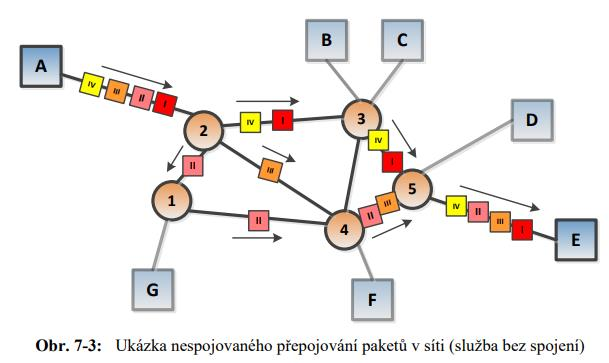
\includegraphics[width=0.7\textwidth]{images/q07_connectionless}
	%\caption{Ukázka nespojovaného přepojování paketů v~síti}
\end{figure}

% NOTE Původně tu byl bod "Vliv velikosti paketů na přepojování", ale nic moc se v něm neříkalo.

\subsection{Služby síťové vrstvy}

\subsubsection{Služby síťové vrstvy na~zdrojové stanici}

Základní službou je \textbf{vytváření paketů}: zapouzdření jednotky vyšší vrstvy, přidání záhlaví (adresy, informace). \textbf{Vyhledání logické adresy} dalšího uzlu: vyhledání cíle pro~první skok s~využitím směrovací tabulky. \textbf{Vyhledání linkové adresy} dalšího uzlu: překlad logické adresy pro~přenos po~fyzickém médiu. \textbf{Rozdělení datagramu} na~menší jednotky v~případě potřeby (pokud je vytvořený paket větší než maximální povolená velikost).

\subsubsection{Služby sítové vrstvy na~směrovači}

\textbf{Kontrola bezchybnosti} přenosu paketu, vyhledání logické a~linkové adresy dalšího prvku, rozdělení datagramu, je-li to v~mezilehých uzlech povoleno.

\subsubsection{Služby síťové vrstvy z~pohledu cílové stanice}

\textbf{Kontrola bezchybnosti} přenosu paketu, \textbf{defragmentace} rozdělených částí a~\textbf{předání vyšší vrstvě}.

\subsection{Další služby síťové vrstvy}

I~když \textbf{řízení chybových stavů} řeší až~transportní vrstva, síťová vrstva obsahuje protokol ICMP/ICMPv6, který řízení chybových stavů částečně poskytuje, např. může zasílat \emph{choke packet} signalizující požadavek o~zpomalení.

\textbf{Kvalita služeb} (\emph{Quality of~Services}) spočívá ve~vyhrazení dostatečné kapacity pro~aplikace, které ji vyžadují (videohovory a~další aplikace běžící v~reálném čase). \textbf{Směrování} umožŇuje dynamicky zjišťovat informace o~vzdálených sítích pro~účely směrování. \textbf{Bezpečnost} nebyla původně vůbec řešena, využívá se IPSec.

\subsection{Služby síťové vrstvy poskytované transportní vrstvě}

\textbf{Přenos datových jednotek} je prováděn z~pohledu transportní vrstvy transparentně. \textbf{Výběr kvality služby} určuje chybovost, dostupnost, spolehlivost, propustnost, zpoždění při~přenosu či řízení. \textbf{Výběr typu}: se~spojením či bez~něj. \textbf{Oznamování chyb} neopravených síťovou vrstvou. \textbf{Dodržení pořadí} datových jednotek, \textbf{řízení toku dat}.

\subsection{IPv4}

IPv4 adresa má délku 32 bitů. Počet všech adres je označován jako \textbf{adresní prostor} s~velikostí $2^{32}$, tj. zhruba čtyři miliardy adres. IPv4 adresy se zapisují jako čtyři čísla v~rozsahu $[0, 255]$ oddělena tečkou, např. \texttt{147.229.71.29}.

\textbf{Maska sítě} rozděluje IP adresu na~adresu sítě a~stanice. Jde o~nepřerušenou řadu bitů zleva, která je reprezentována číslem $[1, 32]$ reprezentujícím počet bitů masky. Adresa \texttt{147.229.71.29/24} znamená síť \texttt{147.229.71.0}, adresu \texttt{0.0.0.29} a~masku \texttt{255.255.255.0}: \texttt{11111111 11111111 11111111 00000000}. Číslo za~lomítkem se označuje jako délka prefixu: prefix \texttt{/18} odpovídá masce \texttt{255.255.192.0}.

V~síti je první adresa rezervovaná pro~síť samotnou a~poslední adresa pro~všesměrové vysílání (pakety jsou doručovány všem v~síti); ostatní adresy mohou být přiřazeny stanicím.

Historicky se adresní prostor IPv4 rozděloval pomocí tříd. V~devadesátých letech se přešlo k~beztřídnímu adresování, což umožnilo prostor rozdělit efektivněji.

\begin{figure}
	\centering
	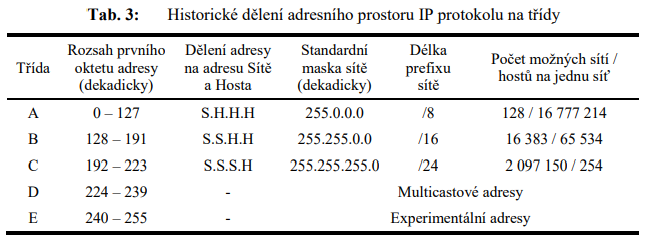
\includegraphics[width=\textwidth]{images/q07_ip_classes}
\end{figure}

\subsubsection{IPv4 datagram}

Při~přenosu je zabalen do~paketu vyšší vrstvy (Ethernet, ATM, \dots). Zabalený datagram zůstává neměnný, s~výjimkou proměnných polí jako hodnota čítače životnosti paketu.

\begin{figure}
	\centering
	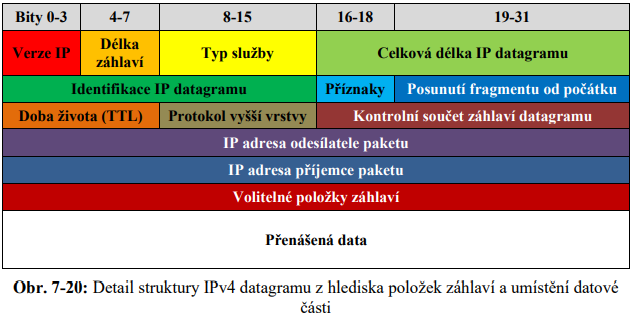
\includegraphics[width=0.7\textwidth]{images/q07_ip_packet}
	\caption*{Verze: \texttt{4}. Délka záhlaví: \texttt{20} až~\texttt{60} v~bajtech. Typ služby: hodnota QoS. }
\end{figure}

\subsection{Směrování}

\clearpage
\section{Síťová vrstva přenosových systémů -- tunelování paketů, ARP, NAT, ICMPv4, IPv6.}

\clearpage
\section{Transportní vrstva přenosových systémů -- služby transportní vrstvy, UDP protokol, TCP protokol.}

\clearpage
\section{Aplikační vrstva přenosových systémů -- DHCP protokol, DNS systém, přenos souborů, webové protokoly, elektronická pošta.}
